\chapter{I. Fázis: Tanítás nélküli tesztelés}
    Ebben a fázisban minden kiválasztott modellt úgy teszteltem a teljes teszthalmazon, hogy nem történt semmiféle finomhangolás vagy tanítás – vagyis a modellek előtanított állapotban, az ImageNet súlyokkal kerültek kiértékelésre.
    
    \textbf{Cél:} A kiindulási teljesítmény meghatározása, amely megmutatja, hogy a modellek milyen mértékben képesek generalizálni az új, de hasonló doménből származó képekre a tanítás nélkül.

    \section{ResNet50}
        \begin{center}
        \begin{longtable}{l c}
        \caption{ResNet50 tanítás nélküli vizsgálat eredményei} \label{tab:phase01_ResNet50} \\
        \toprule
        \textbf{Metrika} & \textbf{Érték} \\
        \midrule
        \endfirsthead
        \toprule
        \textbf{Metrika} & \textbf{Érték} \\
        \midrule
        \endhead
        Top-1 Accuracy & 0.4698 \\
        Top-5 Accuracy & 0.7962 \\
        Precision & 0.3934 \\
        Recall & 0.3797 \\
        F1-score & 0.3592 \\
        Inference time & 25.21 sec \\
        \bottomrule
        \end{longtable}
        \end{center}

        \subsubsection{ResNet50 tanítás nélküli normalizált Confusion Mátrix}
        \begin{figure}[H]
        \centering
        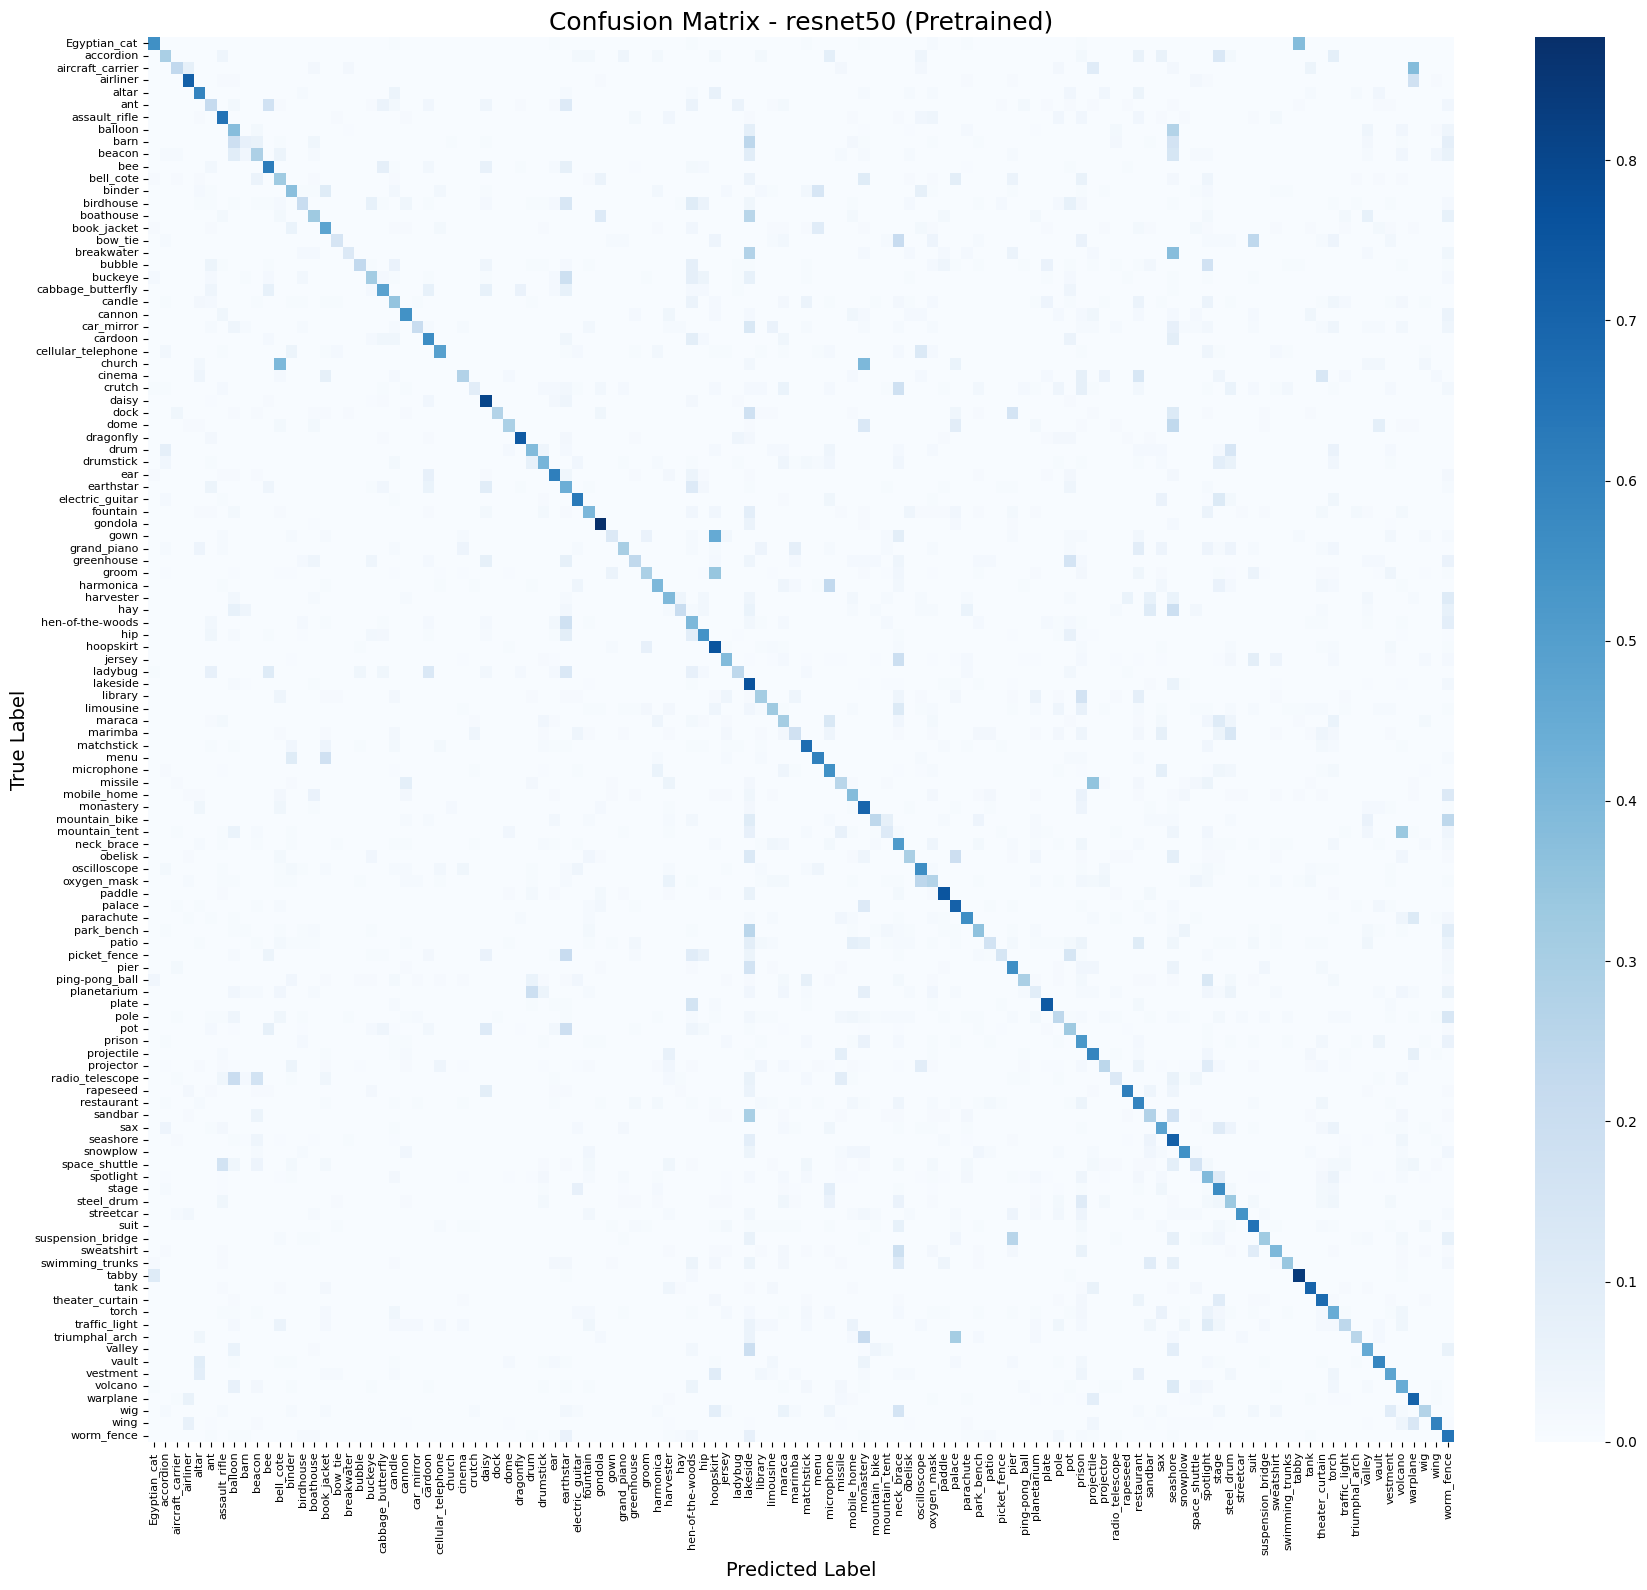
\includegraphics[width=0.8\textwidth]{images/phase01/ResNet50_normalised_conf_mat.png}
        \caption{ResNet50 tanítás nélküli normalizált Confusion Mátrix}
        \label{fig:phase01_ResNet50_normalised_conf_mat}
        \end{figure}

    \section{DenseNet121}
        \subsubsection{DenseNet121 tanítás nélkül teszt}
        \begin{center}
        \begin{longtable}{lc}
        \caption{DenseNet121 @ ImageNet1k tanítás nélküli vizsgálat eredményei}%
        \label{tab:phase01_DenseNet121} \\
        \toprule
        \textbf{Metrika} & \textbf{Érték} \\
        \midrule
        \endfirsthead
        \toprule
        \textbf{Metrika} & \textbf{Érték} \\
        \midrule
        \endhead
        Top-1 Accuracy & 0.4498 \\
        Top-5 Accuracy & 0.7806 \\
        Precision & 0.3874 \\
        Recall & 0.3611 \\
        F1-score & 0.3408 \\
        Inference time & 25.15 sec \\
        \bottomrule
        \end{longtable}
        \end{center}

        \subsubsection{DenseNet121 tanítás nélküli normalizált Confusion Mátrix}
        \begin{figure}[H]
            \centering
            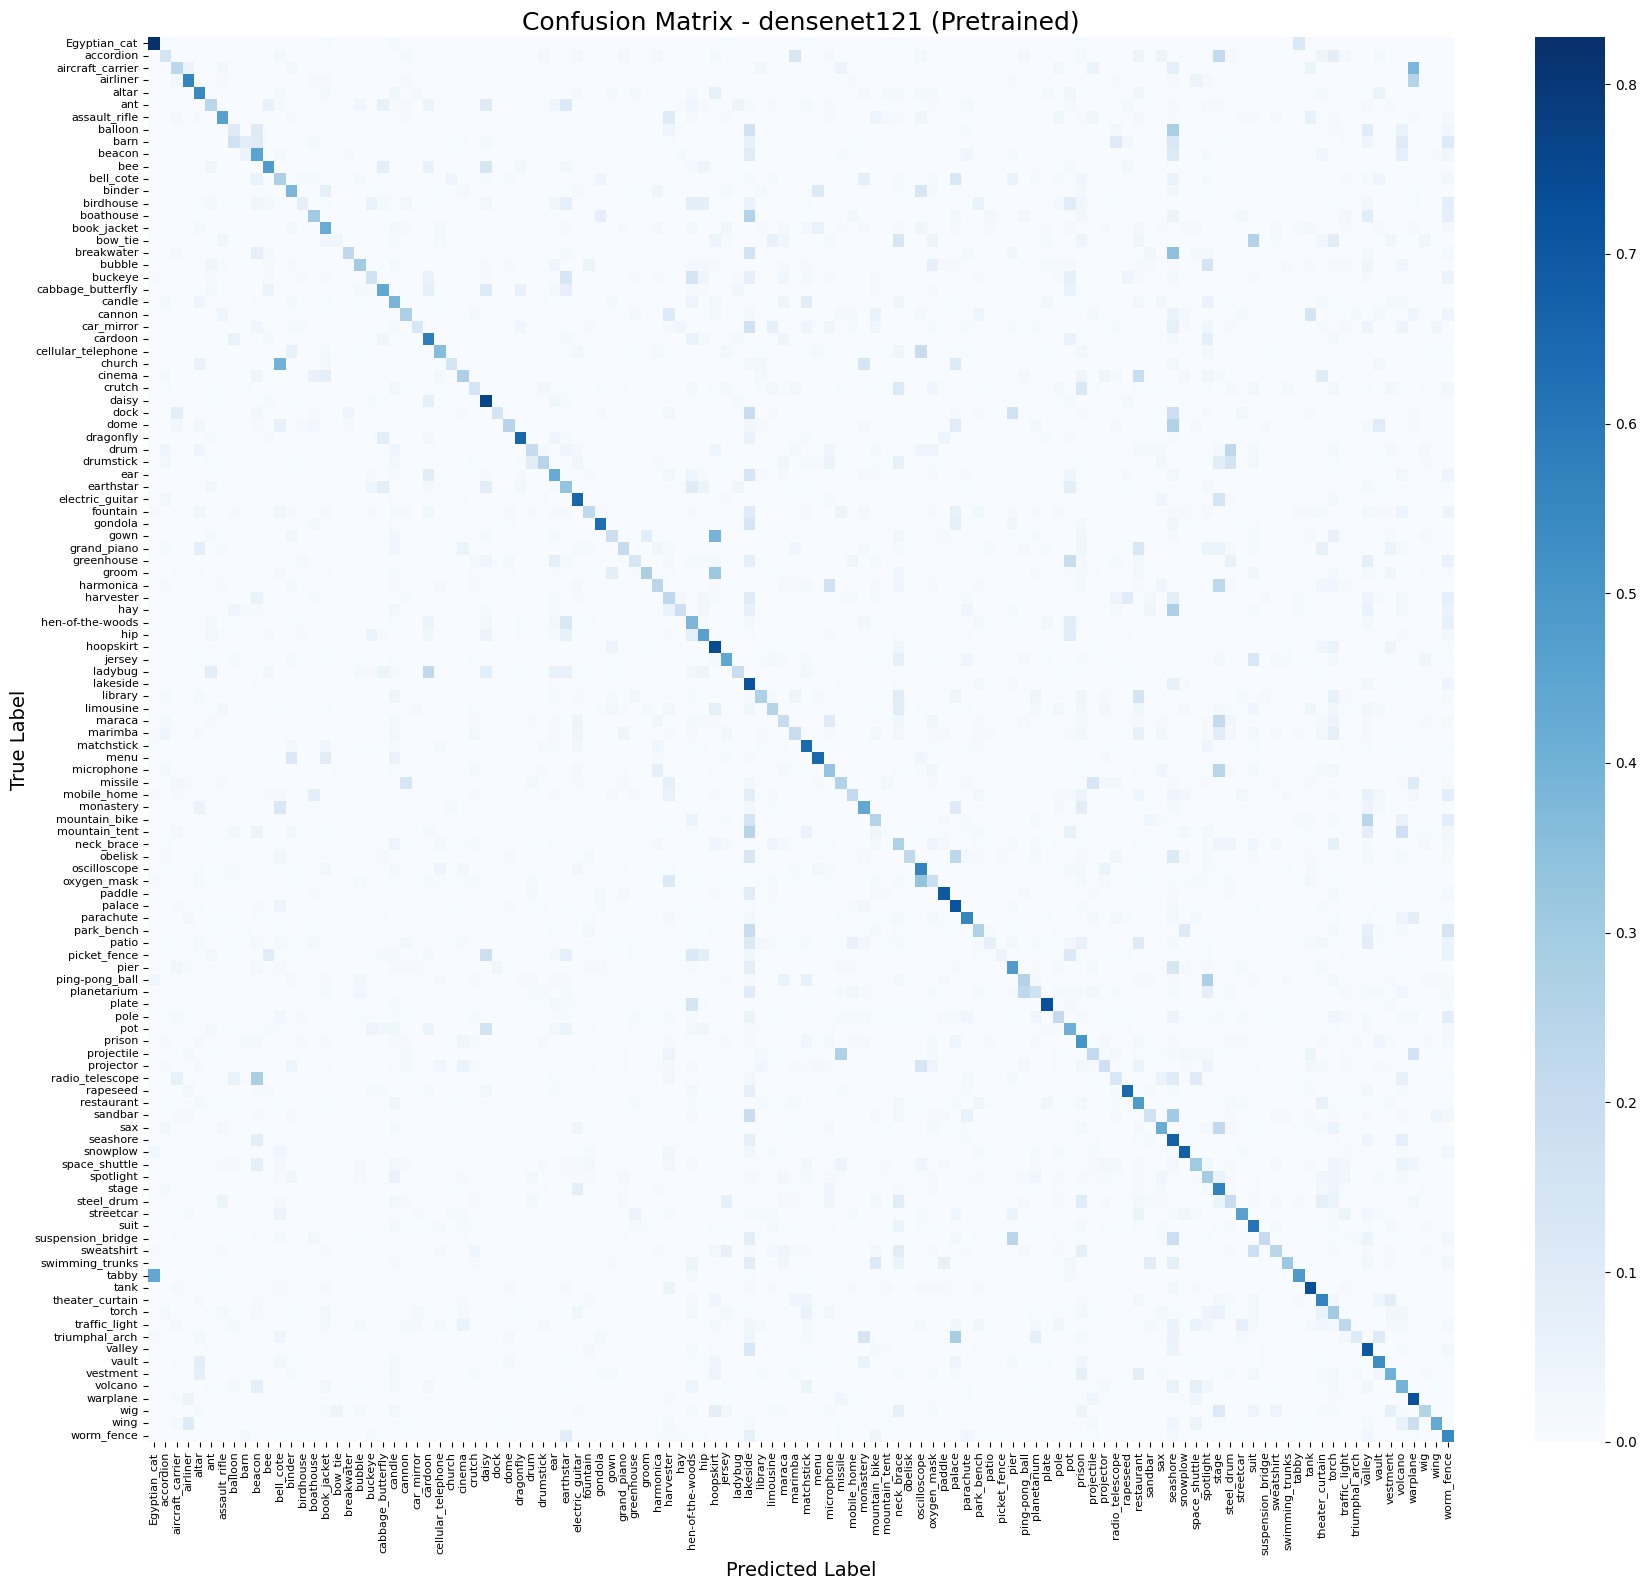
\includegraphics[width=0.8\textwidth]{images/phase01/DenseNet121_normalised_conf_mat.png}
            \caption{DenseNet121 tanítás nélküli normalizált Confusion Mátrix}
            \label{fig:phase01_DenseNet121_normalised_conf_mat}
        \end{figure}

    \section{EfficientNet-B0}
        \subsubsection{EfficientNet-B0 tanítás nélkül teszt}
        \begin{center}
        \begin{longtable}{l c}
        \caption{EfficientNet-B0 tanítás nélküli vizsgálat eredményei} \label{tab:phase01_EfficientNet-B0} \\
        \toprule
        \textbf{Metrika} & \textbf{Érték} \\
        \midrule
        \endfirsthead
        \toprule
        \textbf{Metrika} & \textbf{Érték} \\
        \midrule
        \endhead
        Top-1 Accuracy & 0.4802 \\
        Top-5 Accuracy & 0.8217 \\
        Precision & 0.4137 \\
        Recall & 0.4039 \\
        F1-score & 0.3829 \\
        Inference time & 28.89 sec \\
        \bottomrule
        \end{longtable}
        \end{center}

        \subsubsection{EfficientNet-B0 tanítás nélküli normalizált Confusion Mátrix}
        \begin{figure}[H]
          \centering
          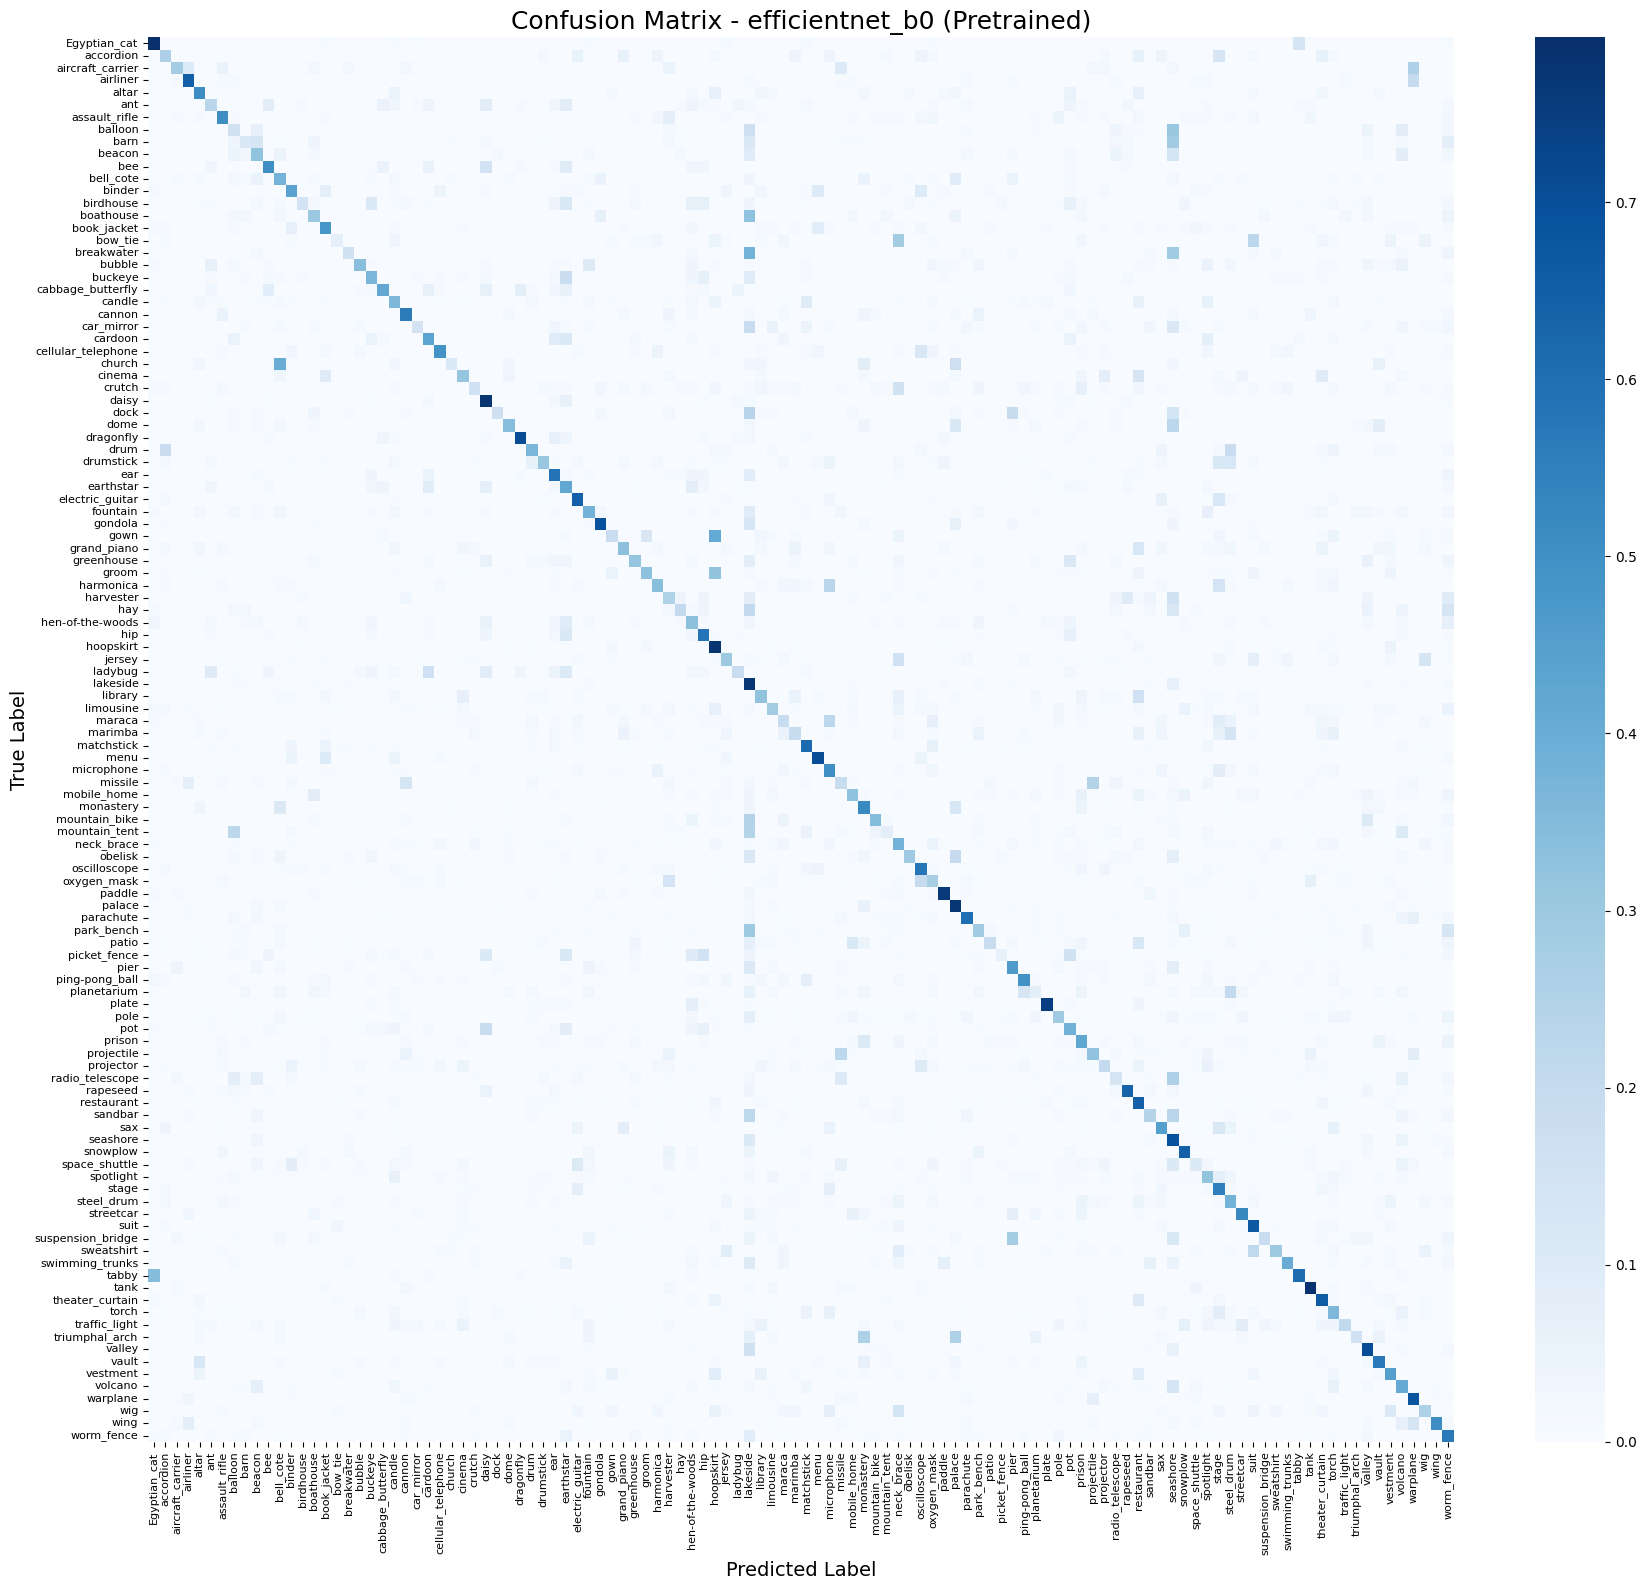
\includegraphics[width=0.8\textwidth]{images/phase01/EfficientNet-B0_normalised_conf_mat.png}
          \caption{EfficientNet-B0 tanítás nélküli normalizált Confusion Mátrix}
          \label{fig:phase01_EfficientNet-B0_normalised_conf_mat}
        \end{figure}

    \section{ConvNeXt-Tiny}
        \subsubsection{ConvNeXt-Tiny tanítás nélkül teszt}
        \begin{center}
        \begin{longtable}{l c}
        \caption{ConvNeXt-Tiny tanítás nélküli vizsgálat eredményei} \label{tab:phase01_ConvNeXt-Tiny} \\
        \toprule
        \textbf{Metrika} & \textbf{Érték} \\
        \midrule
        \endfirsthead
        \toprule
        \textbf{Metrika} & \textbf{Érték} \\
        \midrule
        \endhead
        Top-1 Accuracy & 0.5048 \\
        Top-5 Accuracy & 0.8471 \\
        Precision & 0.4917 \\
        Recall & 0.4369 \\
        F1-score & 0.4194 \\
        Inference time & 38.40 sec \\
        \bottomrule
        \end{longtable}
        \end{center}

        \subsubsection{ConvNeXt-Tiny tanítás nélküli normalizált Confusion Mátrix}
        \begin{figure}[H]
          \centering
          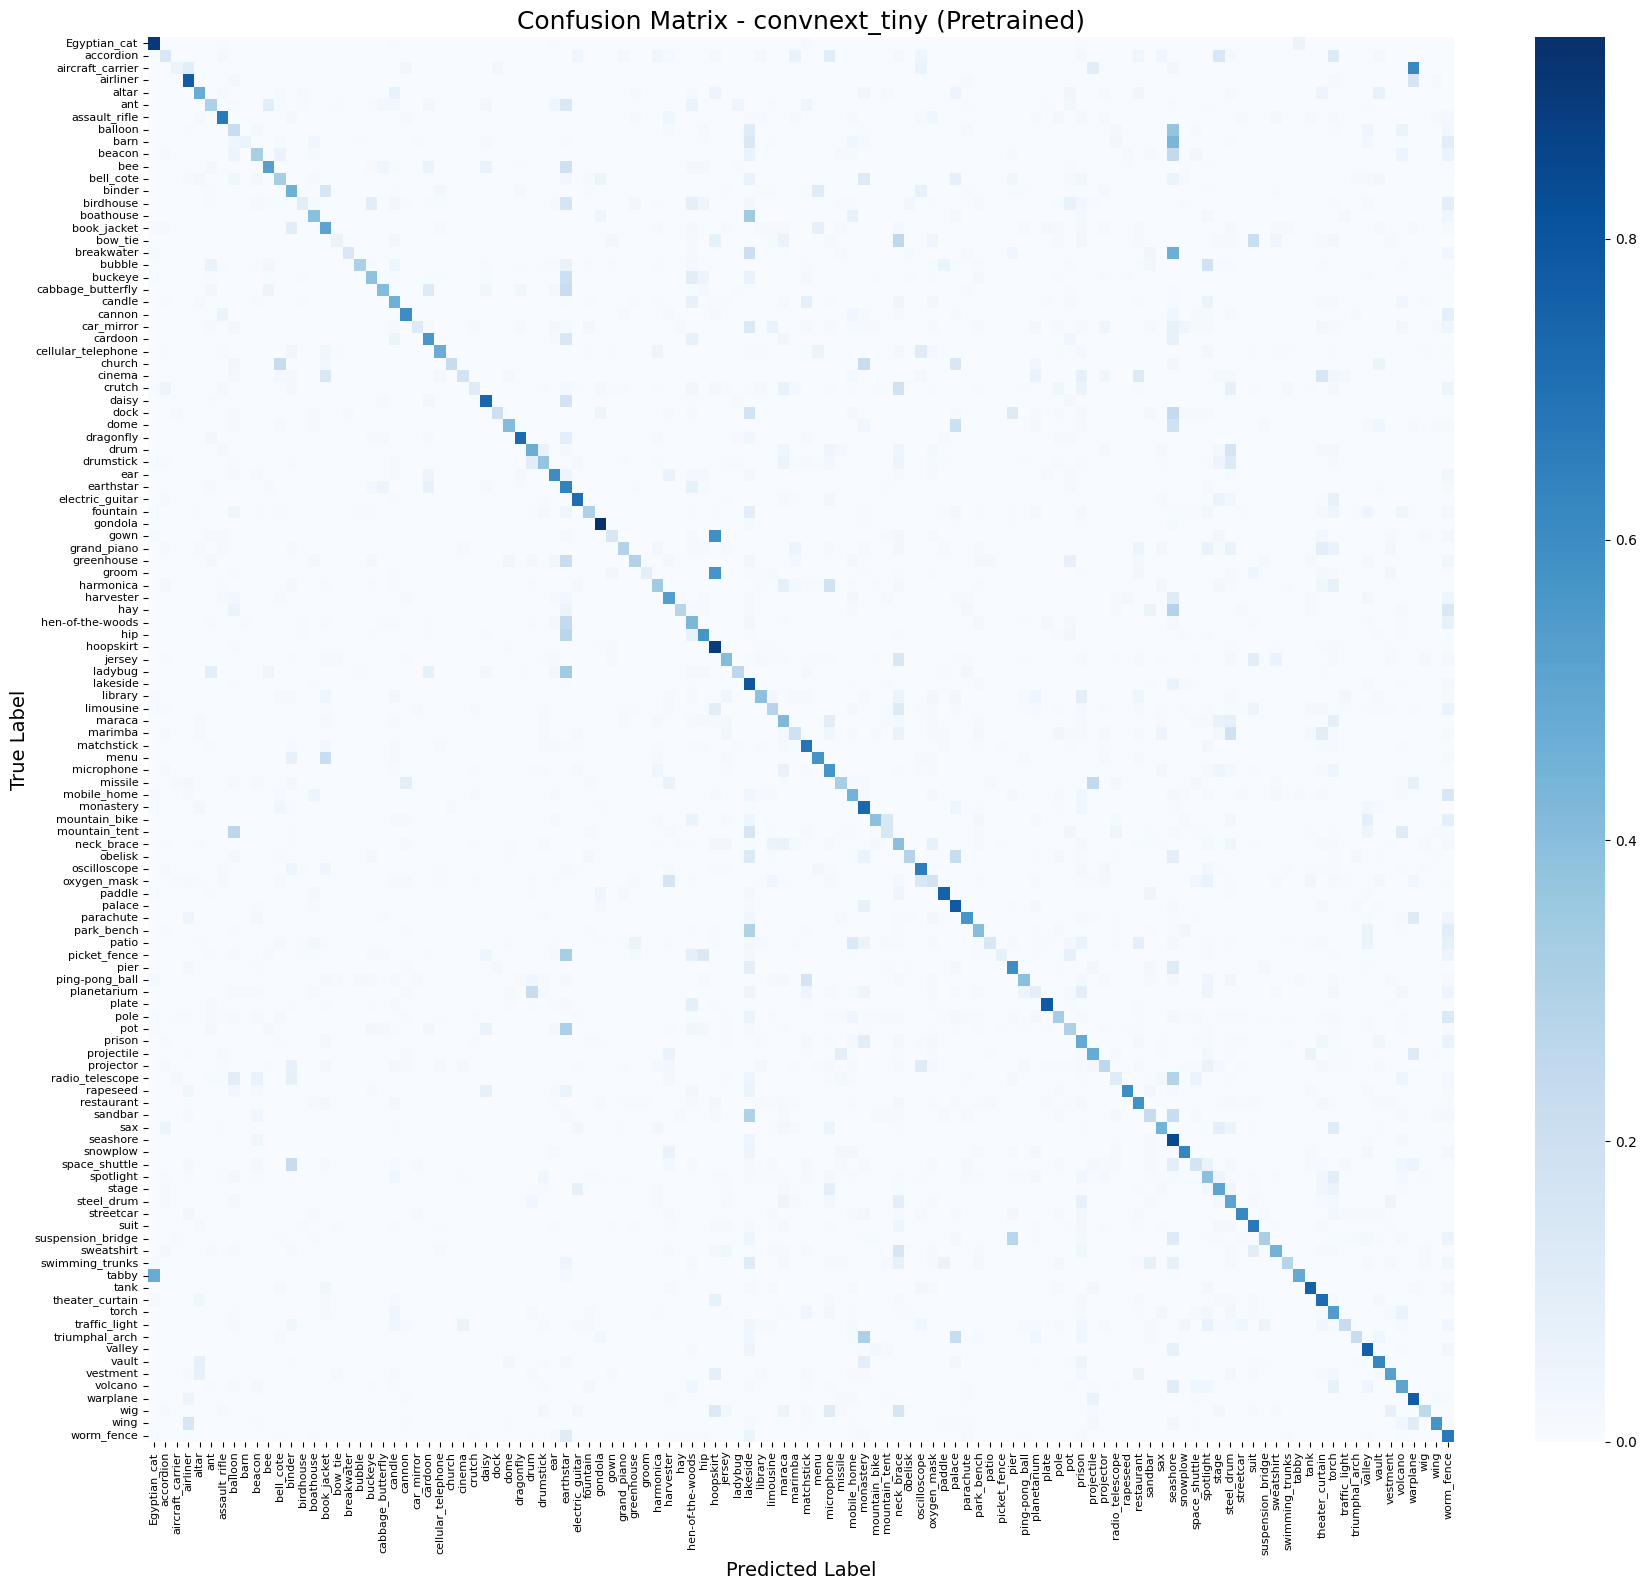
\includegraphics[width=0.8\textwidth]{images/phase01/ConvNeXt-Tiny_normalised_conf_mat.png}
          \caption{ConvNeXt-Tiny tanítás nélküli normalizált Confusion Mátrix}
          \label{fig:phase01_ConvNeXt-Tiny_normalised_conf_mat}
        \end{figure}

    \section{ViT-B/16}
        \subsubsection{ViT-B-16 tanítás nélkül teszt}
        \begin{center}
        \begin{longtable}{l c}
        \caption{ViT-B-16 tanítás nélküli vizsgálat eredményei} \label{tab:phase01_ViT-B-16} \\
        \toprule
        \textbf{Metrika} & \textbf{Érték} \\
        \midrule
        \endfirsthead
        \toprule
        \textbf{Metrika} & \textbf{Érték} \\
        \midrule
        \endhead
        Top-1 Accuracy & 0.5308 \\
        Top-5 Accuracy & 0.8582 \\
        Precision & 0.4629 \\
        Recall & 0.4419 \\
        F1-score & 0.4307 \\
        Inference time & 92.13 sec \\
        \bottomrule
        \end{longtable}
        \end{center}

        \subsubsection{ViT-B-16 tanítás nélküli normalizált Confusion Mátrix}
        \begin{figure}[H]
            \centering
            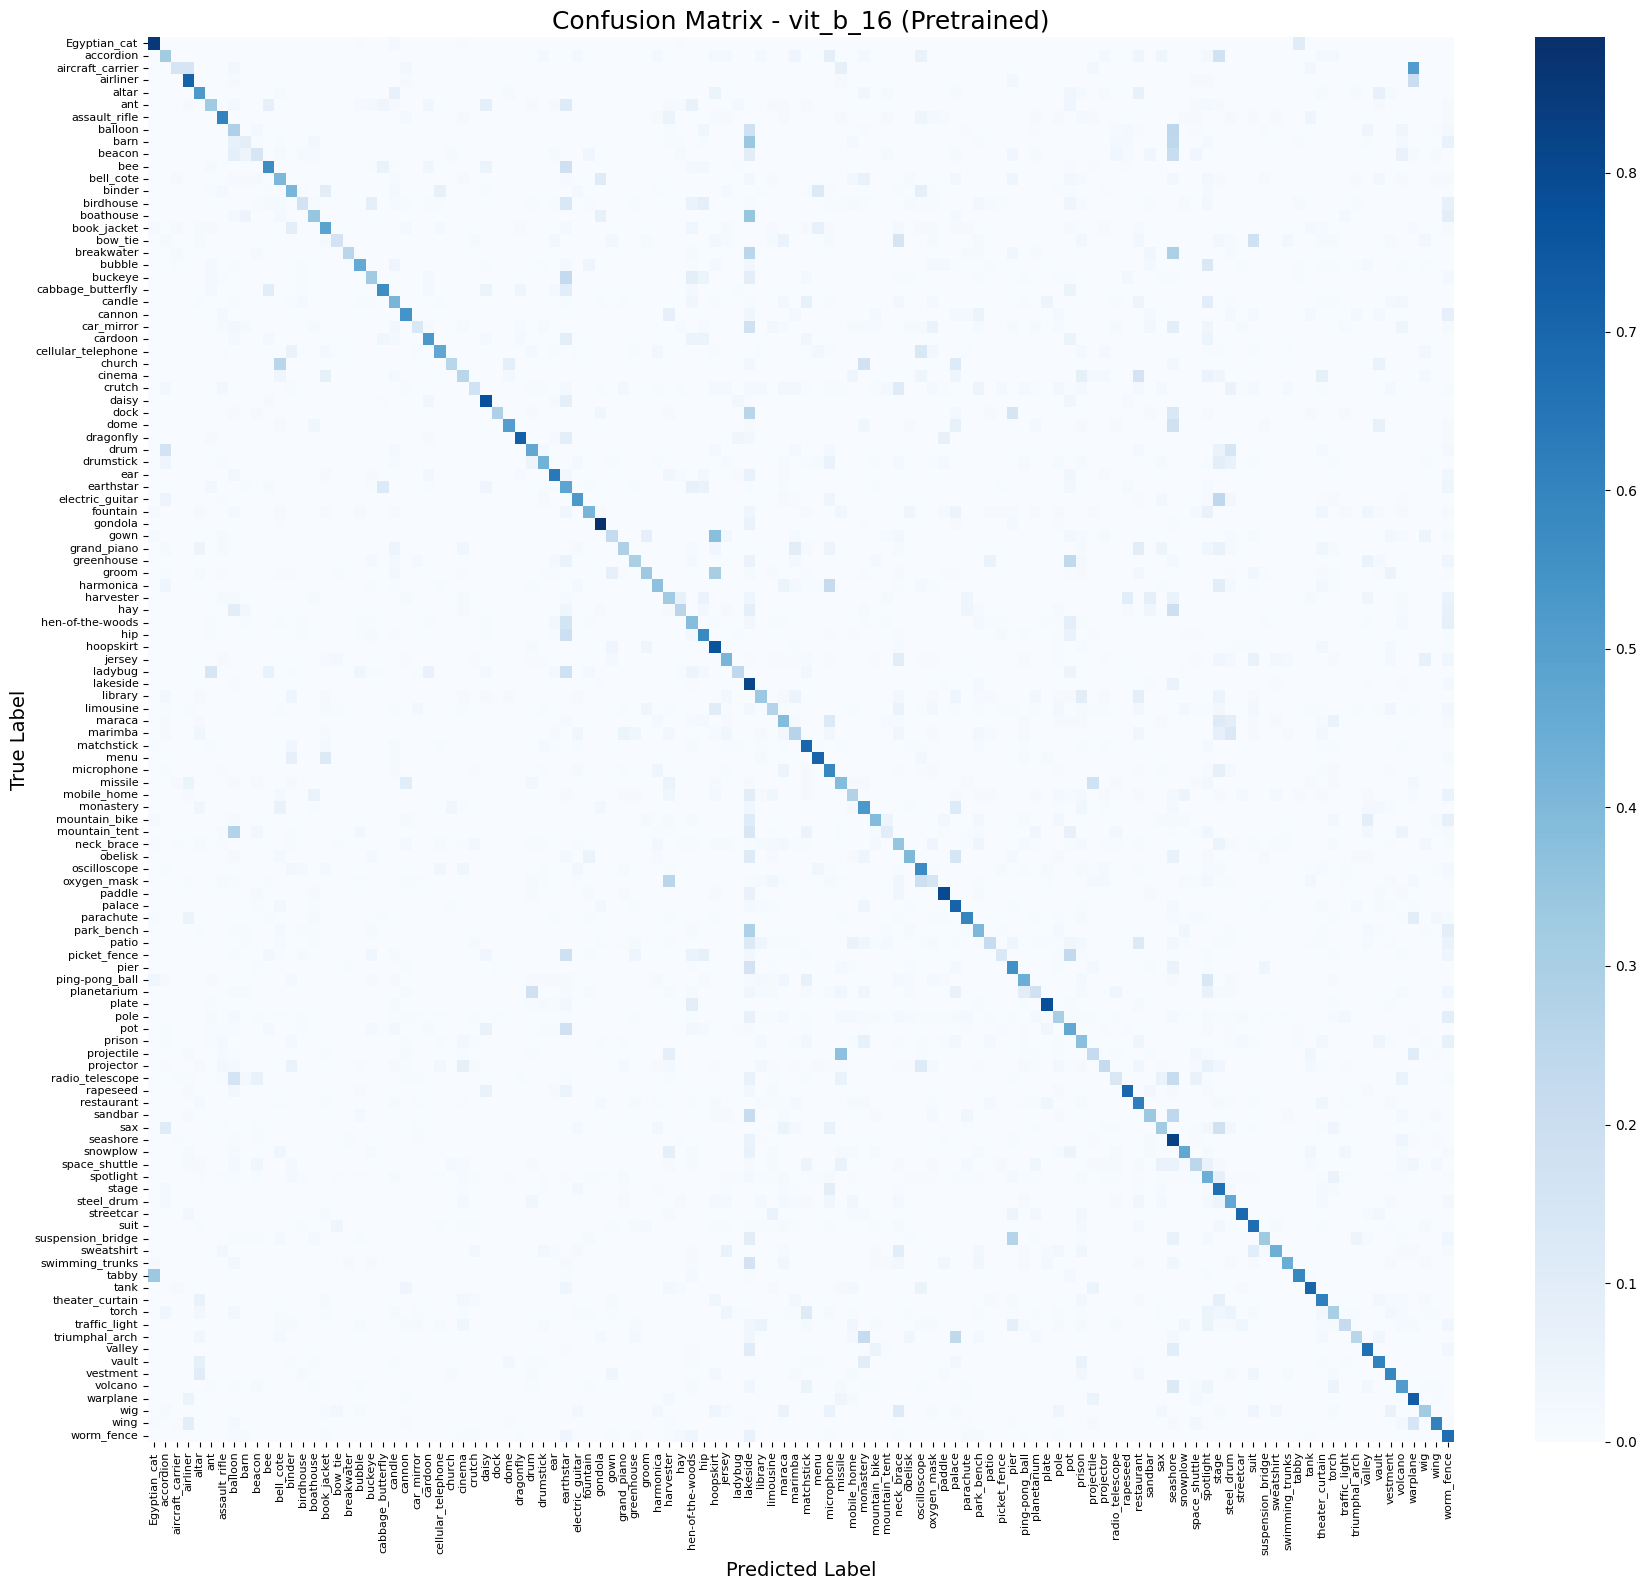
\includegraphics[width=0.8\textwidth]{images/phase01/ViT-B-16_normalised_conf_mat.png}
            \caption{ViT-B-16 tanítás nélküli normalizált Confusion Mátrix}
            \label{fig:phase01_ViT-B-16_normalised_conf_mat}
        \end{figure}

    \section{Inception-v3}
        \subsubsection{Inception-v3 tanítás nélkül teszt}
        \begin{center}
        \begin{longtable}{l c}
        \caption{Inception-v3 tanítás nélküli vizsgálat eredményei} \label{tab:phase01_Inception-v3} \\
        \toprule
        \textbf{Metrika} & \textbf{Érték} \\
        \midrule
        \endfirsthead
        \toprule
        \textbf{Metrika} & \textbf{Érték} \\
        \midrule
        \endhead
        Top-1 Accuracy & 0.4763 \\
        Top-5 Accuracy & 0.8008 \\
        Precision & 0.3833 \\
        Recall & 0.3896 \\
        F1-score & 0.3683 \\
        Inference time & 38.06 sec \\
        \bottomrule
        \end{longtable}
        \end{center}

        \subsubsection{Inception-v3 tanítás nélküli normalizált Confusion Mátrix}
        \begin{figure}[H]
          \centering
          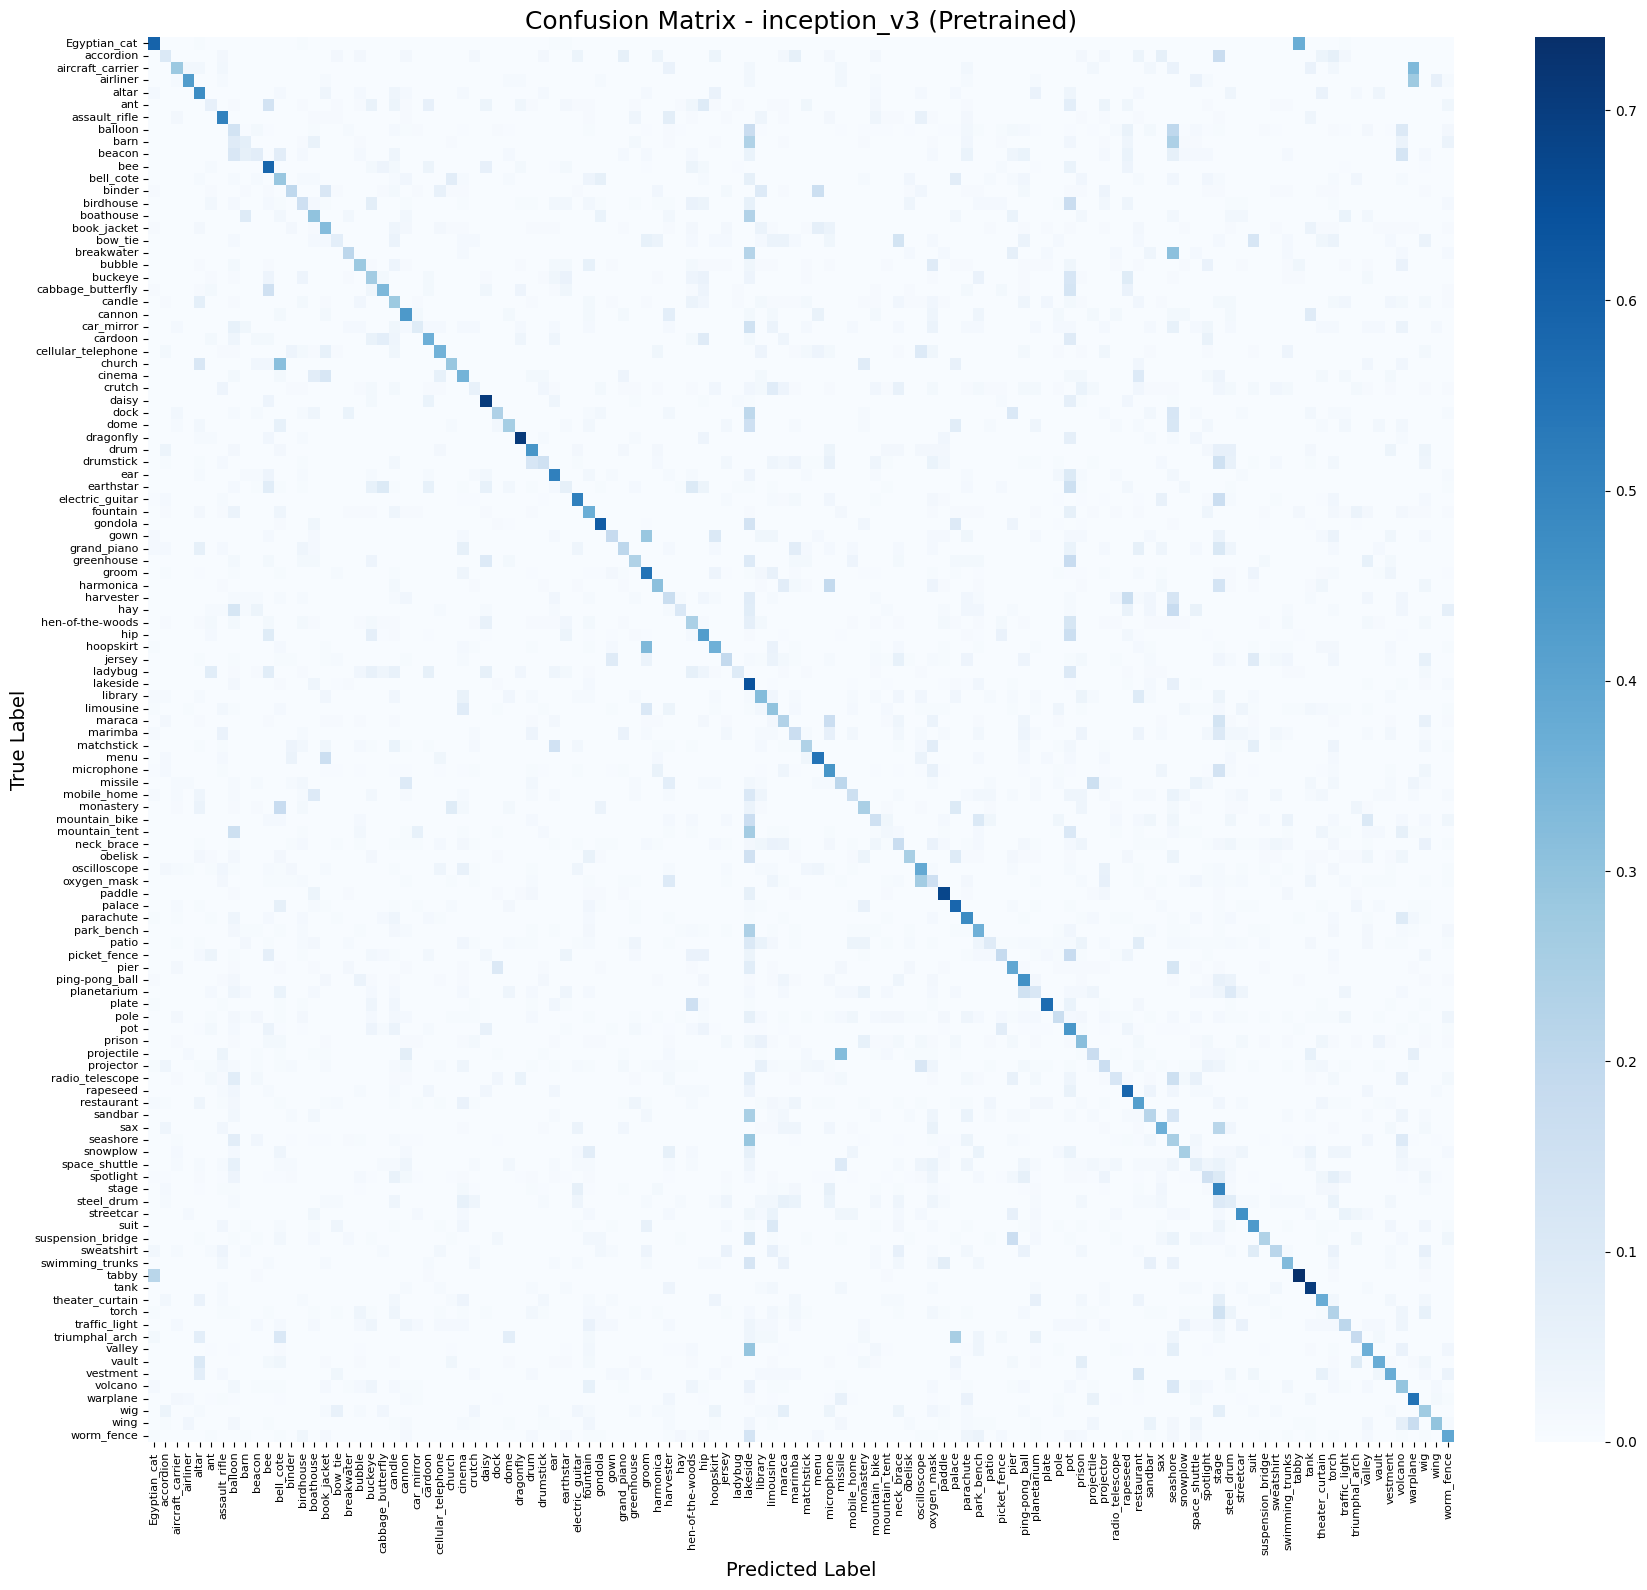
\includegraphics[width=0.8\textwidth]{images/phase01/Inception-v3_normalised_conf_mat.png}
          \caption{Inception-v3 tanítás nélküli normalizált Confusion Mátrix}
          \label{fig:phase01_Inception-v3_normalised_conf_mat}
        \end{figure}

    \section{NASNet}
        \subsubsection{NASNet tanítás nélkül teszt}
        \begin{center}
        \begin{longtable}{l c}
        \caption{NASNet tanítás nélküli vizsgálat eredményei} \label{tab:phase01_NASNet} \\
        \toprule
        \textbf{Metrika} & \textbf{Érték} \\
        \midrule
        \endfirsthead
        \toprule
        \textbf{Metrika} & \textbf{Érték} \\
        \midrule
        \endhead
        Top-1 Accuracy & 0.2820 \\
        Top-5 Accuracy & 0.5408 \\
        Precision & 0.3204 \\
        Recall & 0.2799 \\
        F1-score & 0.2696 \\
        Inference time & 275.30 sec \\
        \bottomrule
        \end{longtable}
        \end{center}

        \subsubsection{NASNet tanítás nélküli normalizált Confusion Mátrix}
        \begin{figure}[H]
          \centering
          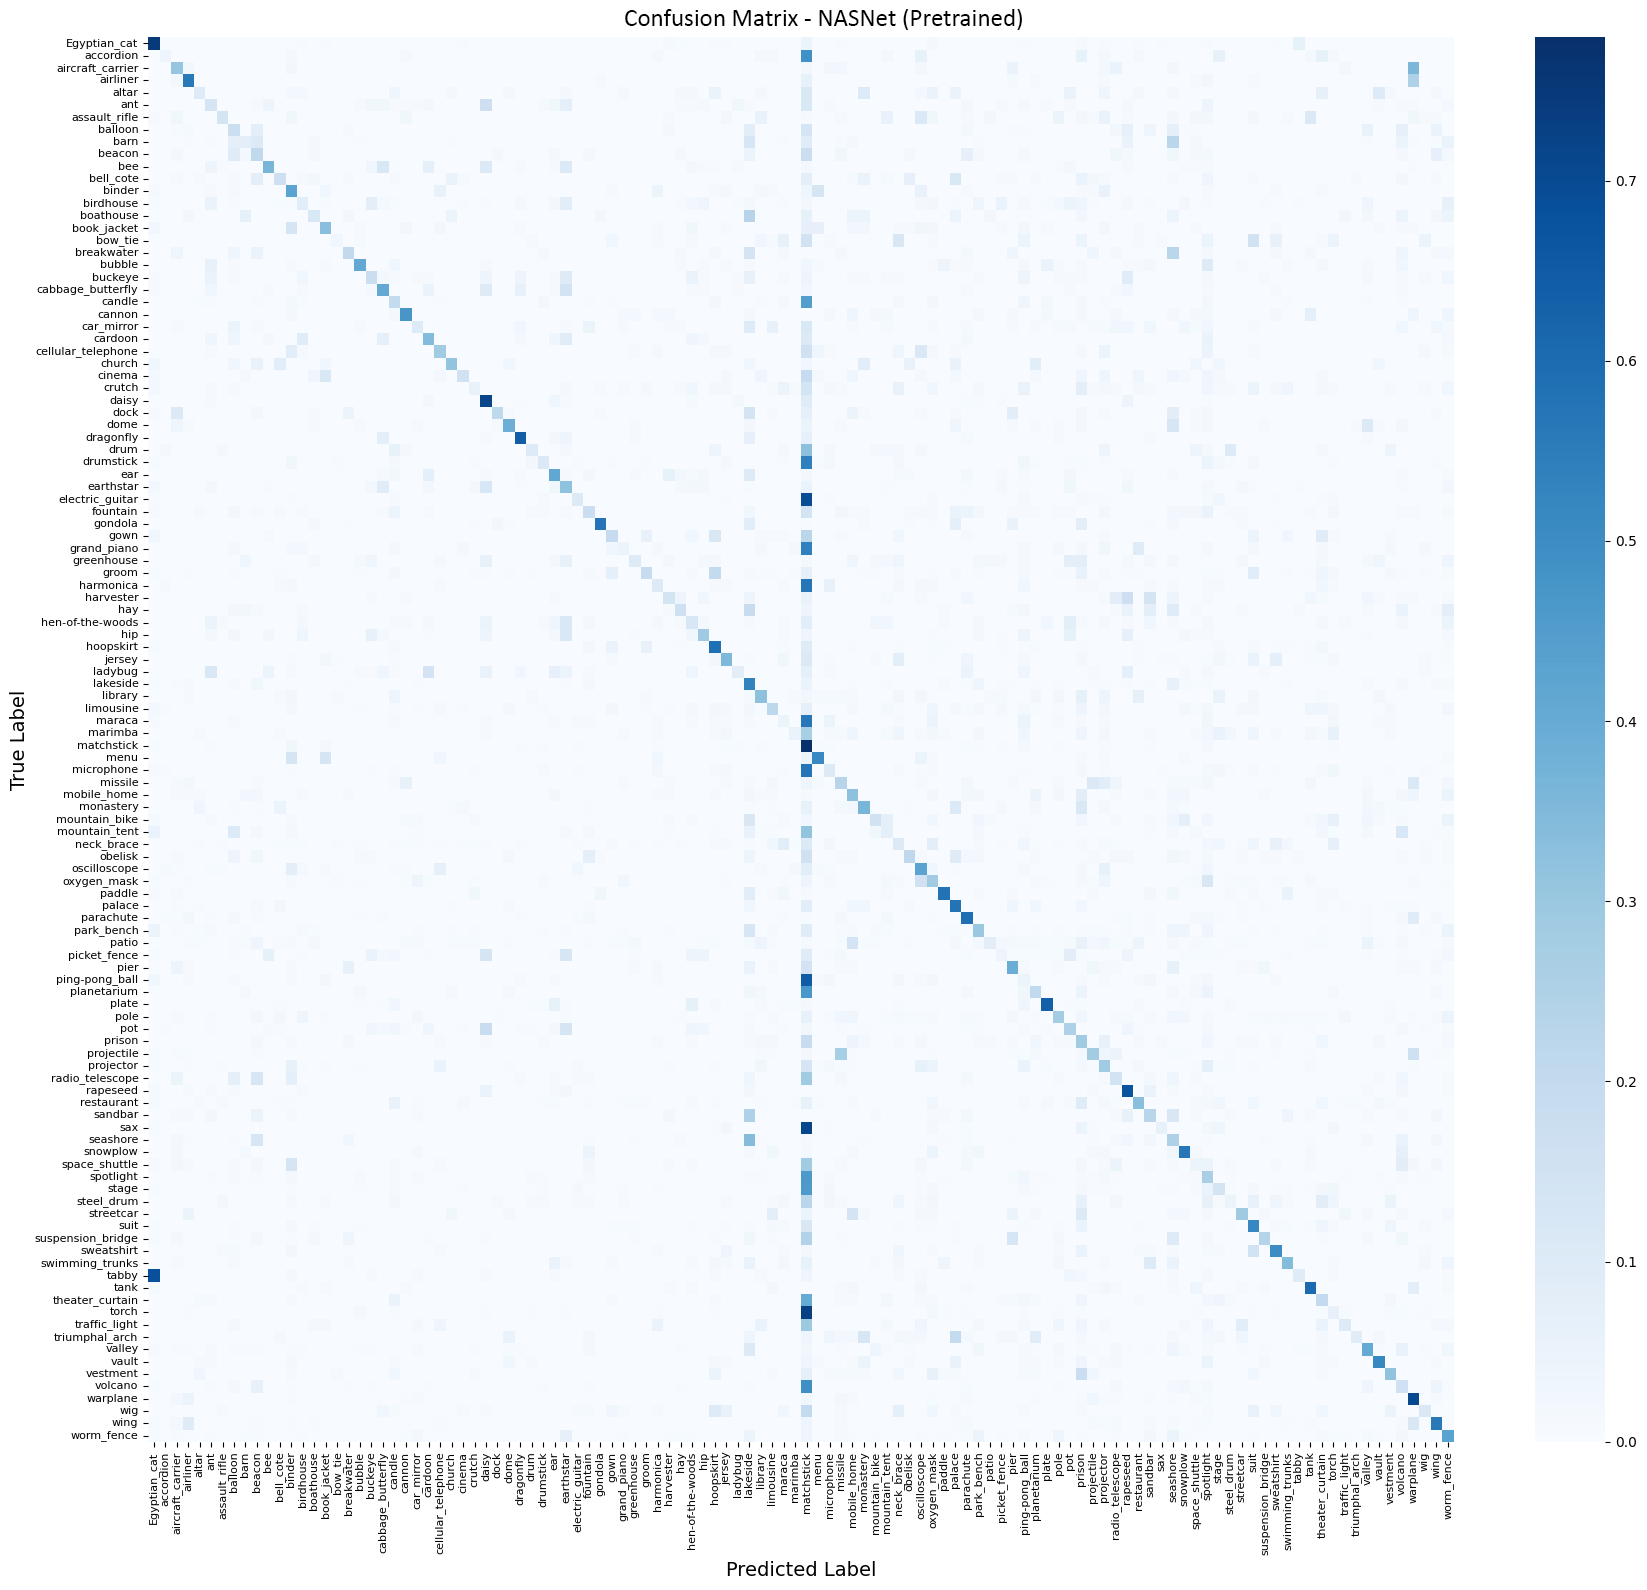
\includegraphics[width=0.8\textwidth]{images/phase01/NASNet_normalised_conf_mat.png}
          \caption{NASNet tanítás nélküli normalizált Confusion Mátrix}
          \label{fig:phase01_NASNet_normalised_conf_mat}
        \end{figure}

    \section{Összefoglaló}

    Összefoglaló az első mérési fázis eredményeiről. A hét ismert modell tanítás nélküli eredeti élsúlyokkal történő vizsgálata történt meg a saját ImageNet1k osztályozású adathalmazomon ami összesen 180750 képet tartalmaz 114 imagenet osztályba sorolva ahol nincs 300 képnél kisebb kategória Train, Val, Test halmazokra osztva 80, 10, 10 arányban. Így a Test halmaz 18172 képet tartalmaz szintén 114 kategóriára osztva. Ezen történt a hét ismert modell első fázisú tesztelése saját tanítás nélküli eredeti ImageNet1k-n előtanított súlyokkal. Nézzük most ennek a vizsgáltnak az eredményeit.


\subsubsection{Összefoglaló táblázat az első fázis mért értékeiről}
    \begin{center}
        \begin{longtable}{lllllll}
        \caption{Modellek összefoglaló értékei tanítás nélkül}\label{tab:phase1_summary_table}\\
        \toprule
        Modell & Top-1 Acc. & Top-5 Acc. & Precision & Recall & F1-score & Idő(s) \\
        \midrule
        \endfirsthead
        \toprule
        Modell & Top-1 & Top-5 & Precision & Recall & F1-score & Idő(s) \\
        \midrule
        \endhead
        ConvNeXt-Tiny & 0.5048 & 0.8471 & 0.4917 & 0.4369 & 0.4194 & 38.40 \\
        ViT-B/16 & 0.5308 & 0.8582 & 0.4629 & 0.4419 & 0.4307 & 92.13 \\
        EfficientNet-B0 & 0.4802 & 0.8217 & 0.4137 & 0.4039 & 0.3829 & 28.89 \\
        ResNet50 & 0.4698 & 0.7962 & 0.3934 & 0.3797 & 0.3592 & 25.21 \\
        DenseNet121 & 0.4498 & 0.7806 & 0.3874 & 0.3611 & 0.3408 & 25.15 \\
        Inception-v3 & 0.4763 & 0.8008 & 0.3833 & 0.3896 & 0.3683 & 38.06 \\
        NASNet & 0.2820 & 0.5408 & 0.3204 & 0.2799 & 0.2696 & 275.30 \\
        \bottomrule
        \end{longtable}
        \end{center}

    \subsubsection{Top 1 és Top 5 pontosságok összehasonlítása modellenként tanítás nélkül.}
        \begin{figure}[H]
            \centering
            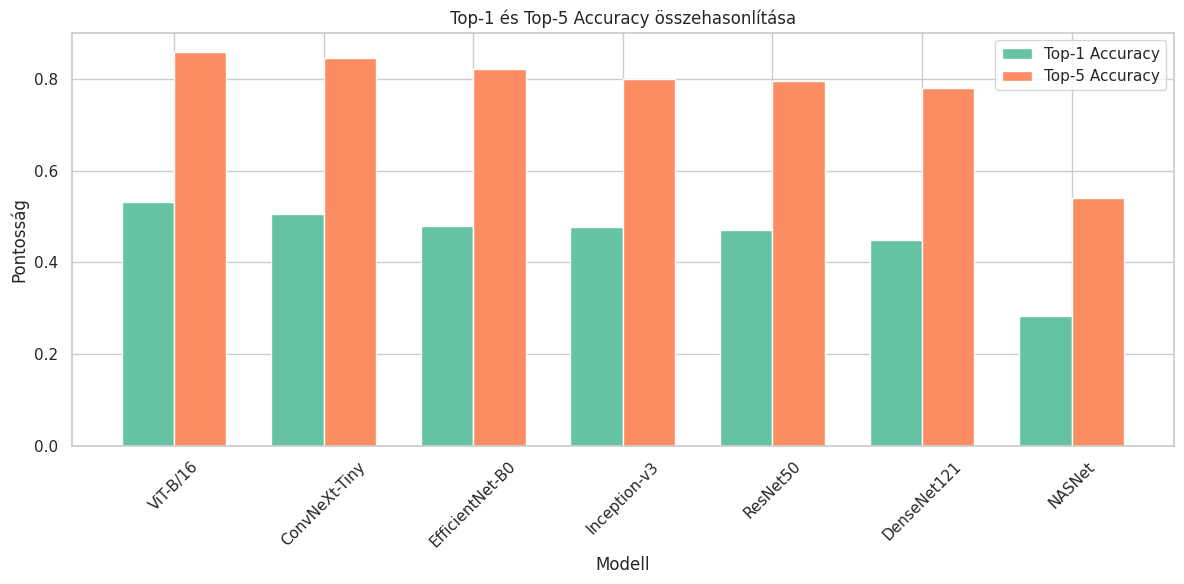
\includegraphics[width=1.0\textwidth]{images/phase01/summary01.png}
            \caption{Top 1 és Top 5 pontosságok összehasonlítása modellenként tanítás nélkül.}
            \label{fig:phase01_summary01}
        \end{figure}

    \subsubsection{Precision, Recall, F1-score összehasonlítása modellenként tanítás nélkül.}
        \begin{figure}[H]
            \centering
            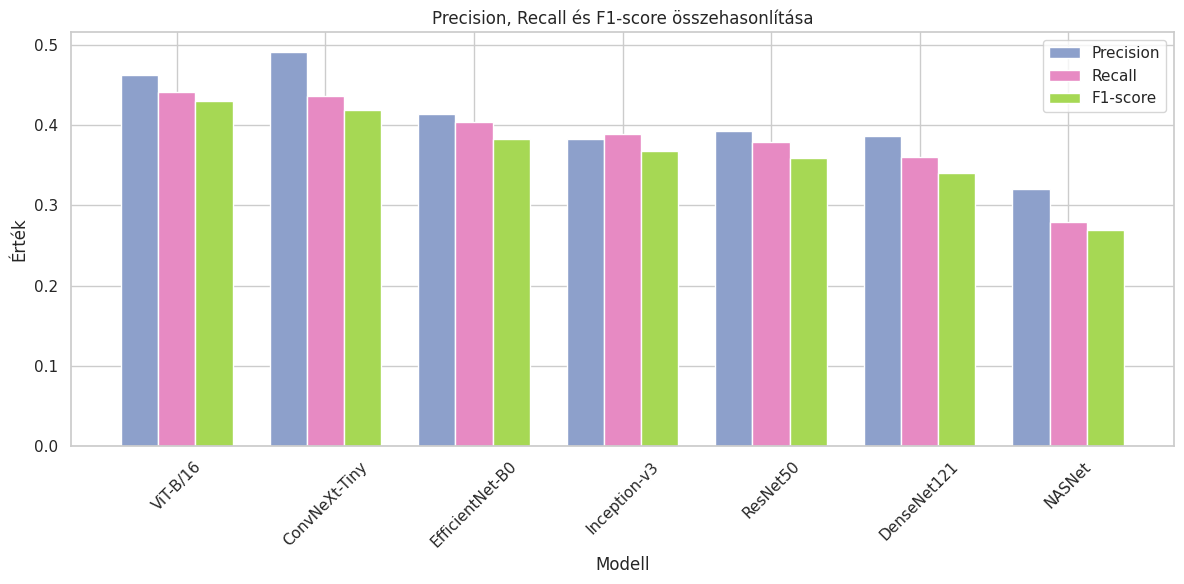
\includegraphics[width=1.0\textwidth]{images/phase01/summary02.png}
            \caption{Precision, Recall, F1-score összehasonlítása modellenként tanítás nélkül.}
            \label{fig:phase01_summary02}
        \end{figure}

    \subsubsection{Teszt lefutási idejének összehasonlítása modellenként tanítás nélkül.}
        \begin{figure}[H]
            \centering
            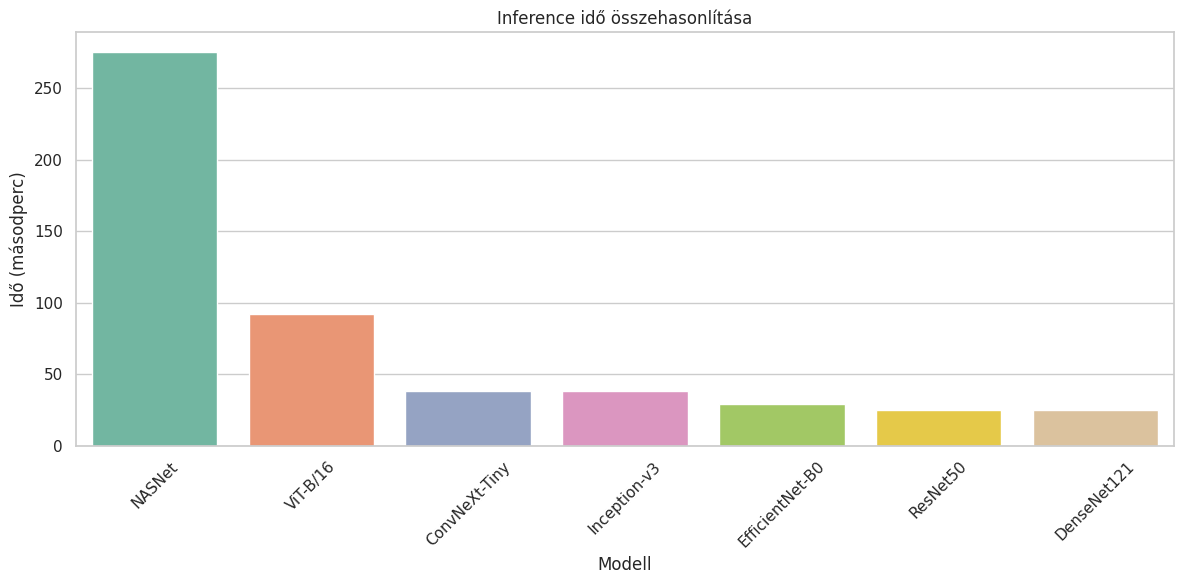
\includegraphics[width=1.0\textwidth]{images/phase01/summary03.png}
            \caption{Teszt lefutási idejének összehasonlítása modellenként tanítás nélkül.}
            \label{fig:phase01_summary03}
        \end{figure}

    \subsubsection{Az első fázis rövid szöveges értékelése}
    Az első mérési fázis során hét különböző, előre betanított modellt teszteltem a saját sb-photothemes-imagenet114 adatbázis 18000 képből álló, 114 kategóriát tartalmazó teszthalmazán. A modelleket itt az első fázisban tanítás nélkül, a gyári súlyokkal értékeltem.

    Pontosság tekintetében a ViT-B/16 modell érte el a legjobb Top-1 (53,08\%) és Top-5 (85,82\%) pontosságot, szorosan követi a ConvNeXt-Tiny és az EfficientNet-B0. Ezek az eredmények azt mutatják, hogy a transformer-alapú és modern CNN architektúrák jobban teljesítenek a hagyományosabb modelleknél, mint például a ResNet50 vagy a DenseNet121. A NASNet jelentősen alacsonyabb pontosságot ért el, ami arra utalhat, hogy nem optimalizált az adott teszthalmazra.

    Precision, Recall és F1-score mutatók alapján a ViT-B/16 és a ConvNeXt-Tiny modellek kiemelkednek, ami megerősíti a pontossági eredményeket. Ezek a modellek nemcsak pontosak, hanem megbízhatóak is a kategóriák felismerésében.

    Inference idő szempontjából a DenseNet121 és a ResNet50 modellek a leggyorsabbak (~25 másodperc), míg a NASNet jelentősen lassabb (275,30 másodperc), ami korlátozhatja a gyakorlati alkalmazhatóságát, különösen valós idejű rendszerekben.

    Összegzésként, a ViT-B/16 és a ConvNeXt-Tiny modellek kínálják a legjobb kompromisszumot a pontosság és a teljesítmény között, bár a ViT-B/16 jelentősen hosszabb inference idővel rendelkezik. A DenseNet121 és a ResNet50 gyorsabbak, de alacsonyabb pontosságot nyújtanak. A NASNet alacsony pontossága és hosszú inference ideje miatt kevésbé ajánlott az adott feladatra.